\chapter{Fehlerkontrolle}
Ziel des Kapitels ist es, einen berechenbaren, verlässlichen und effizienten Fehlerindikator zu finden. Die Erfahrung zeigt, dass die Größe des Winkels zwischen den zwei affinen Hyperflächen, welche von der Approximation auf den Triangulationselementen angenommen werden, ein guter Fehlerindikator sein könnte. Auf dieser Vermutung beruht die Definition des a posteriori (lat. erfahrungsbasiert; im Gegensatz zu a priori) Fehlerschätzers. 

\section{A Posteriori Fehlerschätzer}
Für die Definition des a posteriori  Fehlerschätzers wird eine Größe für die \verb|"|Schärfe\verb|"| der Kante benötigt. Dies liefert uns der Sprung. Je größer dieser, desto \verb|"|schärfer\verb|"| die Kante (Abbildung \ref{sprung}). 
\begin{definition}[Sprung]
	Sei $u_h\in\mathscr{S}^1(\mathscr{T}_h)$ und $S\in\mathscr{S}_h$ mit $S=T_1 \cap T_2$ für $T_1,T_2 \in \mathscr{T}_h$ verschieden, mit äußeren Normalen $n_{T_1,S},n_{T_2,S}$ auf S. Definiere den Sprung von $\nabla u_h$ über S als
	\[
	\llbracket \nabla u_h \cdot n_S\rrbracket = \nabla u_h|_{T_1} \cdot n_{T_1,S} + \nabla u_h|_{T_2} \cdot n_{T_2,S}
	\]
	Setze $\llbracket \nabla u_h \cdot n_S\rrbracket = 0$ für $S\subset \Gamma_D$
\end{definition} 

\begin{figure}[!htbp]
	\begin{center}
		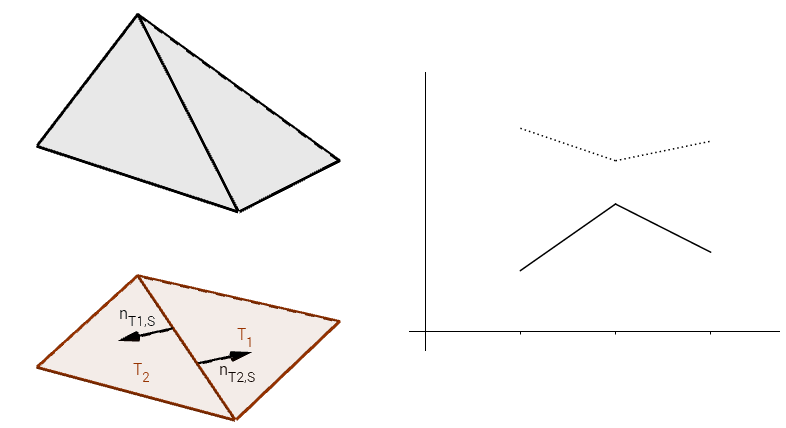
\includegraphics[width=12cm]{pics/Sprung.png}
	\end{center}
	\caption{\label{sprung}Zwei benachbarte Elemente mit darüberliegender Approximation (links) Schnitt entlang der Normalen mit großen (durchgezogene Linie) und kleinem (gestrichelte Linie) Sprung (rechts)}
\end{figure}

\begin{definition}[Verfeinerungsindikator]
	Für $u_h \in \mathscr{S}^1(\mathscr{T}_h) \text{ und } T \in \mathscr{T}_h$, definiere Verfeinerungsindikator $\eta_T(u_h)$ durch
	\[
	\eta^2_T(u_h) = h^2_T\|f\|^2_{L^2(T)} + \sum_{S\in\mathscr{S}_h,S\subset\p T} h_S\|\llbracket \nabla u_h \cdot n_S\rrbracket\|^2_{L^2(S)} \]
\end{definition}
\begin{definition}[Fehlerschätzer]
	Für $u_h \in \mathscr{S}^1(\mathscr{T}_h) \text{ und } \mathscr{T}_h$ definiere den Fehlerschätzer $\eta_\mathscr{R}$ durch
	\[
	\eta_\mathscr{R}^2(u_h)=\sum_{T\in\mathscr{T}_h} \eta^2_T(u_h)
	\]
\end{definition}
Für $u$ Lösungen des Poisson-Problems $-\Delta u = f$ soll nun gezeigt werden, das gilt \\
\begin{center}
	\begin{tabular}{r c l l}
		$\|\nabla(u-u_h)\|$ & $\leq$ & $c_1 \eta_\mathscr{R}(u_h)$ &\textbf{Verlässlichkeit} \\
		$c_2 \eta_\mathscr{R}(u_h)$ &$\leq$& $\|\nabla(u-u_h)\|$ &\textbf{Effiziens} \\
	\end{tabular}
\end{center}
Der Fehlerindikator muss beide dieser Ungleichungen erfüllen. Der triviale Indikator$\eta(u_h)=1$ ist verlässlich aber nicht effizient, während $\eta(u_h)=0$ effizient aber nicht verlässlich ist. Beide sind für die Fehlerkontrolle und als Verfeinerungsindikator ungeeignet.
\section{Lokale Ungleichungen}
Um die Verlässlichkeit zu zeigen, wird ein Resultat über den Clément-Quasi-Interpolanten benötigt. Für dieses Resultat werden zunächst die lokale Poincaré- und lokale Spur-Ungleichung vorgestellt.
\begin{definition}
	Sei $z \in \mathscr{N}_h$ Knoten. Definiere $\omega_z \subset \Omega$ als
	\[
	\omega_z = supp(\varphi_z)
	\]
	Und $h_z = diam(\omega_z)$ Durchmesser von $\omega_z$
\end{definition}
\begin{bemerkung}
	Es gibt $c_{loc} > 0$ so, dass für alle $T \in\mathscr{T}_h, z\in\mathscr{N}_h\cap T$ gilt
	\[
	h_z\leq c_{loc}h_T
	\]
\end{bemerkung}

\begin{lemma}[Lokale Poincaré Ungleichung]
	Sei $v \in H^1_D(\Omega)$ un $z\in \mathscr{N}_h.$ Sei $v_z= 0$ für $z\in \Gamma_D$ und 
	\[ v_z = |\omega_z|^{-1} \int_{\omega_z} v \quad dx
	\]
	sonst. Dann gibt es für alle $h > 0$ und $z \in \mathscr{N}_h$ eine Konstante $c_{p,z}>0$, sodass:
	\[
	\|v-v_z\|_{L^2(\omega_z)}\leq c_{p,z}h_z\|\nabla v\|_{L^2(\omega_z)}.
	\]
\end{lemma}
\textbf{Beweis:}
\begin{itemize}
	\item[i)] 
	Für $z\in \mathscr{N}_h$ sei $\widehat{\omega}_z = h_z^{-1}(\omega_z - z)$. Dann ist nach Konstruktion $diam(\widehat{\omega}_z) = 1$ und
	\[
	\phi_z : \widehat{\omega}_z \rightarrow \omega_z, \quad \hat{x} \mapsto h_z\hat{x}+z
	\]
	affiner Diffeomorphismus mit $D\phi_z = h_zI$.
	
	\begin{figure}[!htbp]
		\begin{center}
			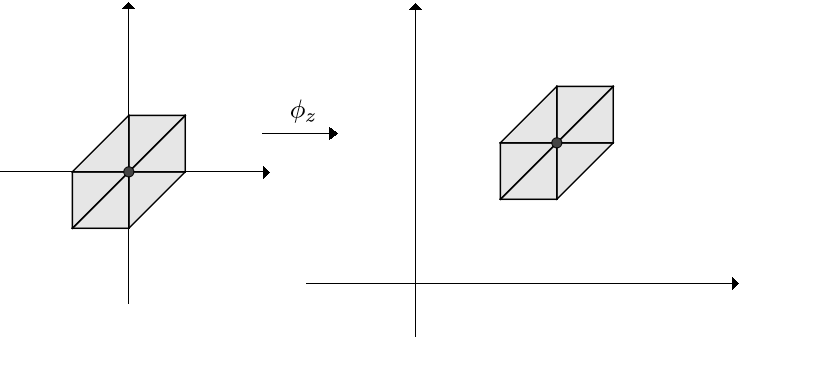
\includegraphics[width=15cm]{pics/omega.png}
		\end{center}
		\caption{Diffeomorphismus $\phi_z$ von $\widehat{\omega}_z$ nach $\omega_z$}
	\end{figure}

	\item[ii)] mit der Standard Poincaré Ungleichung folgt für alle $\widehat{u}\in H^1(\widehat{\omega}_z)$
	\[
	\|\widehat{u}\|_{L^2(\widehat{\omega}_z)} \leq c_{p,z}\|\nabla \widehat{u}\|_{L^2(\widehat{\omega}_z)}
	\]
	wenn \[ \int_{\widehat{\omega}_z}\widehat{u}d\hat{x}=0 \text{ oder }\widehat{u}|_{\hat{\gamma}_z}
	\]
	für geschlossene Teilmenge ${\hat{\gamma}_z} \subset \p \widehat{\omega}_z$ mit positivem Flächenmaß
	\item[iii)] Sei $v_z$ wie im Lemma definiert und $u= v-v_z\in H^1(\omega_z)$, dann erfüllt $\widehat{u} = u \circ \phi_z$ die Bedingungen für die Standard Poincaré Ungleichung auf $\widehat{\omega}_z$
	\item[iv)] Mit der Transformationsformel folgt:
	\begin{eqnarray*}
		\int_{\omega_z} u^2dx&=& \int_{\widehat{\omega}_z} \widehat{u}^2 | detD\phi_z|d\hat{x} \\
		&=& h_z^d\|\widehat{u}\|^2_{L^2(\widehat{\omega}_z)} \leq c^2_{p,z}h^d_z\|\nabla \widehat{u}\|^2_{L^2(\widehat{\omega}_z)} \\
		&=&c^2_{p,z}h^d_z\int_{\widehat{\omega}_z}| \nabla (u\circ\phi_z)|^2 d\hat{x} = c^2_{p,z}h^d_z \int_{\widehat{\omega}_z}|D\phi_z^\top(\nabla u)\circ\phi_z|^2 d\hat{x} \\
		&=& c^2_{p,z}h^d_zh^2_z\int_{\widehat{\omega}_z}|(\nabla u)\circ\phi_z|^2d\hat{x} 
		=c^2_{p,z}h^2_z\int_{\omega_z}|\nabla u|^2dx
	\end{eqnarray*} 
\end{itemize}
$\hfill \Box$

\begin{lemma}[Lokale Spur Ungleichung]
	Sei $S \in  \mathcal{S}_h$ und $T_S \in \mathscr{T}_h$ so, dass $S \subset \p T_s$. Dann
	gibt es die Konstante $c_{Tr} > 0$, sodass für alle $v\in H^1(\Omega)$ gilt:
	\[
	\|v\|^2_{L^2(S)} \leq c^2_{Tr}(h_S^{-1}\|v\|^2_{L^2(T_S)}+h_S\|\nabla v\|^2_{L^2(T_S)}).
	\]
\end{lemma}
\textbf{Beweis:}
Sei $\hat{S}$ die S entsprechende Seite auf dem Referenzelement $\hat{T}$. Auf dem Referenzdreieck gilt die Spurungleichung
\[
\|\hat{v}\|^2_{L^2(\hat{S})} \leq c\|\hat{v}\|_{L^2(\hat{T})}\|\hat{v}\|_{H^1(\hat{T})}
\]
Nach der Transformation auf T
\[
\|v\|^2_{L^2(S)} \leq c\|v\|_{L^2(T)}(\|\nabla v\|_{L^2(T)}+h_S^{-1}\|v\|_{L^2(T)})
\]
Daraus folgt
\[
\|v\|^2_{L^2(S)} \leq c^2(h_S^{-1}\|v\|^2_{L^2(T)}+h_S\|v\|^2_{H^1(T)})
\]
$\hfill \Box$
\section{Clément Quasi Interpolant}
Im Gegensatz zum nodalen Interpolanten wird der Clément Quasi Interpolant über Mittelwerte definiert. Dies führt dazu, dass an Knoten nicht der exakte Wert angenommen wird. Dafür können auch nicht stetige Funktionen interpoliert werden.
\begin{definition}
    Sei $v \in L^1(\Omega) , z \in \mathscr{N}_h$
	\[
	v_z =  \left\{
	\begin{array}{ll}
		|\omega_z|^{-1} \int_{\omega_z} v dx& \text{f\"ur } z \in \mathscr{N}_h \setminus \Gamma_D\\
		0 &  \text{f\"ur } z \in \mathscr{N}_h \cap \Gamma_D
	\end{array}\right.
	\]
	Definiere den Clément Quasi Interpolant$\mathscr{J}_hv \in \mathscr{S}_D^1(\mathscr{T}_h)$ von v als
	\begin{displaymath}
		\mathscr{J}_hv = \sum_{z\in \mathscr{N}_h} v_z \varphi_z
	\end{displaymath}
\end{definition}
\begin{theorem}(Quasi Interpolant Abschätzung)
	Es existiert $c_\mathscr{J} > 0$, so dass f\"ur alle $v\in H^1_D(\Omega)$ gilt:
	\[
	\|\nabla\mathscr{J}_hv\| +\|h^{-1}_\mathscr{T}(v-\mathscr{J}_hv)\| +\|h^{-\frac{1}{2}}_\mathscr{S}(v-\mathscr{J}_hv)\|_{L^2(\cup\mathscr{S}_h)} \leq c_\mathscr{J}\|\nabla v\|
	\]
	mit $h_\mathscr{T}: \Omega \rightarrow  \R \text{ und } h_\mathscr{S}: \cup \mathscr{S}_h \rightarrow  \R$, definiert durch $h_\mathscr{T}|_T = h_T \text{ und }  h_\mathscr{S}|_S = h_S$ \\ f\"ur alle $T\in\mathscr{T}_h, S\in\mathscr{S}_h$ 
\end{theorem}
\textbf{Beweis:}
\begin{itemize}
	\item[i)] Da $\sum_{\varphi\in\mathscr{N}_h}\varphi_z = 1$ in $\Omega$ ist $\sum_{z\in\mathscr{N}_h}\nabla \varphi_z=0$
	\[
	\nabla \mathscr{J}_hv = \nabla \sum_{z\in \mathscr{N}_h}v_z\varphi_z = \sum_{z\in \mathscr{N}_h}(v_z-v) \nabla\varphi_z
	\]
	da $supp(\varphi_z)=\omega_z$
	\begin{eqnarray*}
		\| \nabla \mathscr{J}_hv\| &=& \int_{\Omega}(\sum_{z\in \mathscr{N}_h}(v_z-v) \nabla\varphi_z)\cdot \nabla \mathscr{J}_hvdx\\
		&\leq& \sum_{z\in \mathscr{N}_h}\int_{\omega_z}|v_z-v| |\nabla\varphi_z||\nabla \mathscr{J}_hv|dx
	\end{eqnarray*}
Die Inversenabschätzung liefert für alle z
\[
\|\nabla\varphi_z\|_{L^\infty(\omega_z)}\leq c_{inv}h^{-1}_z\|\varphi_z\|_{L^\infty(\omega_z)} =c_{inv}h^{-1}_z.
\]
Mit Hölder-,Cauchy-Schwarz- und der lokalen Poincaréungleichung folgt
\begin{eqnarray*}
	\|\nabla\mathscr{J}_hv\|^2 &\leq&\sum_{z\in \mathscr{N}_h}\|v_z-v\|_{L^2(\omega_z)} \|\nabla\varphi_z\|_{L^\infty(\omega_z)}\|\nabla \mathscr{J}_hv\|_{L^2(\omega_z)}\\
	&\leq&c_{inv}c_p\sum_{z\in \mathscr{N}_h}\|\nabla v\|_{L^2(\omega_z)} \|\nabla \mathscr{J}_hv\|_{L^2(\omega_z)} \\
	&\leq&c_{inv}c_p(\sum_{z\in \mathscr{N}_h}\|\nabla v\|_{L^2(\omega_z)}^2)^{1/2} (\sum_{z\in \mathscr{N}_h} \|\nabla \mathscr{J}_hv\|_{L^2(\omega_z)}^2)^{1/2} \\
	&\leq&c_{inv}c_p(d+1)\|\nabla v\| \|\nabla \mathscr{J}_hv\|
\end{eqnarray*} 
In der letzten Abschätzung folgt aus endlicher Überlappung der $\omega_z$
\[
\sum_{z\in \mathscr{N}_h}\|\nabla v\|_{L^2(\omega_z)}^2 \leq (d+1)\sum_{T\in\mathscr{T}_h} \|\nabla v\|^2_{L^2(T)} = (d+1)\|\nabla v\|^2
\]
Teilen durch $\|\nabla\mathscr{J}_hv\|$ liefert die erste Abschätzung
\item[ii)] Für beliebiges $\psi \in L^2(\Omega)$ gilt
\begin{eqnarray*}
	\int_{\Omega}\psi(v-\mathscr{J}_hv)dx &=& \int_{\Omega}\psi(v-\sum_{z\in \mathscr{N}_h}v_z\varphi_z)dx \\
	 &=& \int_{\Omega}\psi(\sum_{z\in \mathscr{N}_h}v\varphi_z-\sum_{z\in \mathscr{N}_h}v_z\varphi_z)dx\\
	 &=&\sum_{z\in \mathscr{N}_h}\int_{\omega_z} \psi (v-v_z)\varphi_zdx \\
	 &\leq&\sum_{z\in \mathscr{N}_h}\int_{\omega_z} |\psi| |v-v_z|dx \\
	 &\leq&c_p \sum_{z\in \mathscr{N}_h}\|\psi\|_{L^2(\omega_z)}h_z\|\nabla v\|_{L^2(\omega_z)}\\
	 &\leq&c_pc_{loc}\sum_{z\in \mathscr{N}_h}\|h_{\mathscr{T}}\psi\|_{L^2(\omega_z)}\|\nabla v\|_{L^2(\omega_z)}\\
	  &\leq&c_pc_{loc}(d+1)\|h_{\mathscr{T}}\psi\|\|\nabla v\|
\end{eqnarray*}
Durch geschicktes Wählen von $\psi = h_{\mathscr{T}}^{-2}(v-\mathscr{J}_hv)$ folgt die zweite Abschätzung
\item[iii)]
Für $S\in\mathscr{S}_h$ und $T_S\in\mathscr{T}_h$ so, dass $S\subset\p T_S$. Mit der lokalen Spurungleichung folgt
\begin{eqnarray*}
	\|h_{\mathscr{S}}^{1/2}(v-\mathscr{J}_hv)\|^2_{L^2(\cup \mathscr{S}_h)} &=& \sum_{S\in\mathscr{S}_h} h_S^{-1}\|v-\mathscr{J}_hv\|^2_{L^2(S)}\\
	 &=&c^2_{Tr} \sum_{S\in\mathscr{S}_h} (h_S^{-2}\|v-\mathscr{J}_hv\|^2_{L^2(T_S)} +
	 \|\nabla (v-\mathscr{J}_hv)\|^2_{L^2(T_S)})\\
	 &\leq&dc^2_{Tr} \sum_{T\in\mathscr{T}_h} (c_{loc}^2h_T^{-2}\|v-\mathscr{J}_hv\|^2_{L^2(T)} + \|\nabla (v-\mathscr{J}_hv)\|^2_{L^2(T)})\\
	 &=&dc^2_{Tr} (c_{loc}^2\|h_{\mathscr{T}}^{-2}(v-\mathscr{J}_hv)\|^2+ \|\nabla (v-\mathscr{J}_hv)\|^2)\\
	 &\leq&dc^2_{Tr}(c_{loc}^2c_1^2+c_2^2)\|\nabla v\|^2.
\end{eqnarray*}
liefert die dritte Abschätzung.
$\hfill \Box$
\end{itemize}
\section{Verlässlichkeitsabschätzung}
Mit Hilfe des Quasi Interpolanten lässt sich nun die erste Abschätzung zeigen, die für die Fehlerkontrolle notwendig ist.
\begin{theorem}[Verlässlichkeitsabschätzung]
	Sei $u\in H^1_0(\Omega)$ schwache Lösung des Poisson-Problems \[-\Delta u = f ,\quad \Gamma_D = \p \Omega \text{ und } u|_{\p \Omega} = 0, \] und $u_h \in \mathscr{S}^1_0(\mathscr{T}_h)$ Galerkin-Approximation von u. Dann gibt es $c_R > 0$ , sodass:
	\[\|\nabla(u-u_h)\|\leq c_R\eta_\mathscr{R}(u_h)
	\]
\end{theorem}
\textbf{Beweis:}
Sei $e = u-u_h$ der Approximationsfehler. Dann folgt aus der Galerkinorthogonalität und da u schwache Lösung des Possoinproblems ist
\begin{eqnarray*}
	\|\nabla e\|^2 &=& \int_{\Omega}\nabla e \cdot \nabla (e-\mathscr{J}_he)dx \\
	&=&\int_{\Omega} \nabla u \cdot \nabla (e-\mathscr{J}_he)dx -\int_{\Omega} \nabla u_h \cdot \nabla (e-\mathscr{J}_he)dx \\
	&=&\int_{\Omega} f (e-\mathscr{J}_he)dx -\int_{\Omega} \nabla u_h \cdot \nabla (e-\mathscr{J}_he)dx
\end{eqnarray*}
Da $\cup T = \Omega$,  $u|_T$ affin und somit $\Delta u|_T=0$ für alle $T\in\mathscr{T}_h$ ist , ergibt sich mit partieller Integration
\begin{eqnarray*}
	\int_{\Omega}\nabla u_h\cdot\nabla (e-\mathscr{J}_he) dx &=& \sum_{T\in\mathscr{T}_h} \int_{T} \nabla u_h \cdot \nabla (e-\mathscr{J}_he) dx \\
	&=& \sum_{T\in\mathscr{T}_h} \left(\int_{T} (-\Delta u_h) (e-\mathscr{J}_he) dx +\int_{\p T} (\nabla u_h \cdot n_T) (e-\mathscr{J}_he) ds\right) \\
	&=&\sum_{T\in\mathscr{T}_h} \int_{\p T} (\nabla u_h \cdot n_T) (e-\mathscr{J}_he) ds
\end{eqnarray*}
In der Summe wird über jede innere Seite zwei mal integriert mit $u_h$ bezüglich der anliegenden Elemente und inversen Normalen. $(e-\mathscr{J}_he)$ ist bezüglich beider Elemente auf der Seite gleich. Da $(e-\mathscr{J}_he)|_{\p \Omega}=0$ und aus der Definition vom Sprung, folgt
\[
\sum_{T\in\mathscr{T}_h} \int_{\p T} (\nabla u_h \cdot n_T) (e-\mathscr{J}_he) ds =
\sum_{S\in\mathscr{S}_h} \int_{S} \llbracket \nabla u_h \cdot n_S\rrbracket (e-\mathscr{J}_he) ds
\]
Mit Hölder- und Schwarz Ungleichungen folgt
\begin{eqnarray*}
	\|\nabla e\|^2 &=&  \sum_{T\in\mathscr{T}_h} \int_{T} f (e-\mathscr{J}_he)dx - \sum_{S\in\mathscr{S}_h} \int_{S} \llbracket \nabla u_h \cdot n_S\rrbracket (e-\mathscr{J}_he) ds \\
	&\leq&  \sum_{T\in\mathscr{T}_h}\|f\|_{L^2(T)} \|e-\mathscr{J}_he\|_{L^2(T)} + \sum_{S\in\mathscr{S}_h} \|\llbracket \nabla u_h \cdot n_S\rrbracket\|_{L^2(S)} \|e-\mathscr{J}_he\|_{L^2(S)}\\
	&\leq& \left( \sum_{T\in\mathscr{T}_h}h_T^2\|f\|_{L^2(T)}^2\right)^{1/2}\left( \sum_{T\in\mathscr{T}_h}h_T^{-2}\|e-\mathscr{J}_he\|_{L^2(T)}^2\right)^{1/2} \\
	&&+ \left(\sum_{S\in\mathscr{S}_h} h_S\|\llbracket \nabla u_h \cdot n_S\rrbracket\|_{L^2(S)}^2\right)^{1/2} \left(\sum_{S\in\mathscr{S}_h}h_S^{-1}\|e-\mathscr{J}_he\|_{L^2(S)}^2\right)^{1/2}\\
	&\leq& \left( \sum_{T\in\mathscr{T}_h}h_T^2\|f\|_{L^2(T)}^2\right)^{1/2}\|h_{\mathscr{T}_h}^{-1}e-\mathscr{J}_he\| \\
	&&+ \left(\sum_{S\in\mathscr{S}_h} h_S\|\llbracket \nabla u_h \cdot n_S\rrbracket\|_{L^2(S)}^2\right)^{1/2} \|h_{\mathscr{S}_h}^{-1/2}e-\mathscr{J}_he\|_{L^2(\Cup \mathscr{S}_h)}
\end{eqnarray*}
Mit der Quasi Interpolanten Abschätzung und der Ungleichung $a+b\leq \sqrt{2(a^2+b^2)}$ folgt

\begin{eqnarray*}
 \|\nabla e\| &\leq& c_{\mathscr{J}}\left( \sum_{T\in\mathscr{T}_h}h_T^2\|f\|_{L^2(T)}^2\right)^{1/2}
+ c_{\mathscr{J}}\left(\sum_{S\in\mathscr{S}_h} h_S\|\llbracket \nabla u_h \cdot n_S\rrbracket\|_{L^2(S)}^2\right)^{1/2} \\
 &\leq& \sqrt{2}c_{\mathscr{J}}\left( \sum_{T\in\mathscr{T}_h}h_T^2\|f\|_{L^2(T)}^2
 + \sum_{S\in\mathscr{S}_h} h_S\|\llbracket \nabla u_h \cdot n_S\rrbracket\|_{L^2(S)}^2\right)^{1/2}
\end{eqnarray*}
$\hfill \Box$
\section{Effizienz}
Für die Effizienzabschätzung werden zunächst Hilfsaussagen über die sogenannten Bubble Funktionen bewiesen.
\begin{definition}
	Für $S \in \mathscr{S}_h$ Seite, definiere 
	\[
		\omega_S= int(\bigcup_{T\in\mathscr{T}_h,S\subset \p T}T)
    \]
    und für ein Element $T \in \mathscr{T}_h$ definiere
    \[
    \omega_T = \bigcup_{z\in\mathscr{N}_h,z\in T} \omega_z
    \]
\end{definition}
\begin{lemma}
	\leavevmode
	\begin{itemize}
		\item[1)]
		Für alle $T\in\mathscr{T}_h$ mit $T =conv\{z_1,z_2,...,z_{d+1}\}$ gibt es Konstanten $c_{e,1},c_{e,2}>0$,  sodass für die \textsf{Element Bubble-Funktion} $b_T = \varphi_{z_1}\varphi_{z_2}\cdots\varphi_{z_{d+1}} \in H^1(\Omega)\cap C(\overline{\Omega})$ gilt:
		\[
		supp(b_T)\subset T,\quad \int_{T} b_T =c_{e,1} |T|, \quad \|\nabla b_T\|_{L^2(T)} \leq c_{e,2}h_T^{d/2-1}
		\]
		\item[2)]
		Für alle $S\in\mathscr{S}_h$ mit $S =conv\{z_1,z_2,...,z_{d}\}$ gibt es Konstanten $c_{s,1},c_{s,2}>0$,  sodass für die \textsf{Seiten Bubble-Funktion} $b_S = \varphi_{z_1}\varphi_{z_2}\cdots\varphi_{z_{d}} \in H^1(\Omega)\cap C(\overline{\Omega})$ gilt:
		\[
		supp(b_S)\subset \omega_S,\quad \int_{S} b_S =c_{s,1} |S|, \quad \|\nabla b_S\|_{L^2(\omega_S)} \leq c_{s,2}h_S^{d/2-1}
		\]
	\end{itemize}
\end{lemma}
\textbf{Beweis:}
\begin{itemize}
	\item[i)] Damit $b_T\neq0$ müssen alle $\varphi_{z_{i}}\neq 0$. Somit folgt\[
	supp(b_T) = \cap_{i=1}^{d+1}supp(\varphi_{z_i})\subset T
	\]
	\item[ii)] Mit der Standard-Integralabschätzung folgt \[
	\int_{T}b_T \leq \max_{x\in T}b_T \int_{T}1 dx \leq |T|
	\]
	\item[iii)] Mit Standardabschätzung folgt \[
	\|b_T\| \leq \left(\int_{T}b_T^2dx\right)^{1/2} \leq \sqrt{|T|}\leq h_T^{d/2}
	\] Weiter gilt mit der Transformationsformel auf das Referenzelement $\hat{T}$
	\begin{eqnarray*}
		\|\nabla b_T\|^2 &=& \int_{\hat{T}} |\nabla b_{T}\circ \phi_z|^2 | detD\phi_z|d\hat{x} = h_T^dh^{-2}_T\int_{\hat{T}} |\nabla (b_T\circ \phi_z)|^2 d\hat{x} \\
		&=& h^{-2}_T h_T^d\| \nabla \widehat{b}_{\hat{T}}\|_{L^2(\hat{T})}^2 \leq c h^{-2}_T h_T^d \|\widehat{b}_{\hat{T}}\|_{L^2(\hat{T})}^2 \\
		&=& ch^{-2}_T\int_{\hat{T}} | (b_T\circ \phi_z)|^2 | detD\phi_z| d\hat{x}= ch^{-2}_T \| b_T\|^2
	\end{eqnarray*}
	Mit beiden Ungleichungen folgt die Behauptung.
\end{itemize}
für $b_S$ analog
$\hfill \Box$
\begin{figure}[!htbp]
	\begin{center}
		\includegraphics[width=16cm]{pics/bubble.png}
	\end{center}
	\caption{Bubble-Funktion $b_T$ auf einem Element(links) $b_S$ auf den an S anliegenden Elementen (rechts)}
\end{figure}
\newpage
Die Eigenschaften der Bubble-Funktionen nutzend, ist es nun möglich auch die zweite Ungleichung zur Fehlerkontrolle zu beweisen. 
\begin{theorem}[Lokale Effizienz]
	Sei $d=2, \Gamma_D = \p \Omega$ und $f\in L^2(\Omega)$ elementeweise konstant. Dann existiert eine Konstante $c_E > 0$, sodass für alle $T\in\mathscr{T}_h$ gilt
	\[
		c_E \eta_T^2(u_h)\leq \|\nabla (u-u_h)\|^2_{L^2(\omega_T)}
	\] 
\end{theorem}
\textbf{Beweis:}
\begin{itemize}
	\item[i)] 
	Für $T =conv\{z_1,z_2,...,z_{d+1}\} \in\mathscr{T}_h$ und $b_T = \varphi_{z_1}\varphi_{z_2}\cdots\varphi_{z_{d+1}}$ , dann gilt mit partieller Integration und $\Delta u_h|_T = 0, b_T|_{\p T} = 0$:
	\[
	\int_{\Omega} \nabla (u - u_h) \cdot \nabla b_Tdx =\int_{\Omega} f b_T dx
	\]
    f ist konstant auf T mit Wert $f_T$ und Vorzeichen $\sigma_T$ dann gilt
    \[
    \sigma_T\int_{T}f_Tb_Tdx=|f_T|\int_{T}b_Tdx=c_{e,1}|f_T||T|= c_{e,1}|T|^{1/2}\|f_T\|_{L^2(T)}
    \]
    Mit $c_{loc}h_T \leq |T|^{1/2}$, Hölderungleichung und $\|\nabla b_T\|_{L^2(T)} \leq c_{e,2}$ folgt
    \[
    h_T\|f\|_{L^2(T)}\leq \frac{c_{e,1}}{c_{loc}} |T|^{1/2}\|f\|_{L^2(T)} =\frac{\sigma_T}{c_{loc}}\int_{T}\nabla (u - u_h) \cdot \nabla b_Tdx \leq c_{el} \|\nabla (u-u_h)\|_{L^2(T)}
    \]
    \item[ii)]
    Für $S =conv\{z_1,z_2,...,z_{d}\} = T_1 \cap T_2$ und $b_S = \varphi_{z_1}\varphi_{z_2}\cdots\varphi_{z_{d}}$ , dann gilt mit partieller Integration und $\Delta u_h|_{T_j} = 0, b_T|_{\p T_j\setminus S} = 0$:
    \begin{eqnarray*}
    	\int_{\omega_S} \nabla (u-u_h)\cdot \nabla b_S dx &=& \int_{\omega_S} fb_Sdx -\left(\int_{T_1} \nabla u_h\cdot \nabla b_S dx + \int_{T_2} \nabla u_h\cdot \nabla b_S dx\right) \\
    	&=& \int_{\omega_S} fb_Sdx - \left(\int_{S} (\nabla u_h\cdot n_{T_1}) b_S ds + \int_{S} (\nabla u_h\cdot n_{T_2}) b_S ds\right)\\
    	&=& \int_{\omega_S} fb_Sdx - \int_{S} \llbracket \nabla u_h \cdot n_S\rrbracket b_S ds
    \end{eqnarray*}
    $\llbracket \nabla u_h \cdot n_S\rrbracket$ ist konstant auf S. Sei $\sigma_S$ Vorzeichen von $\llbracket \nabla u_h \cdot n_S\rrbracket$. Dann gilt
    \[
    \sigma_S \int_{S} \llbracket \nabla u_h \cdot n_S\rrbracket b_S ds = c_{S,1}|\llbracket \nabla u_h \cdot n_S\rrbracket||S| =c_{S,1}\|\llbracket \nabla u_h \cdot n_S\rrbracket\|_{L^2(S)}|S|^{1/2}
    \] 
	Mit Hölder-Ungleichung und $\|\nabla b_S\|_{L^2(\omega_S)} \leq c_{S,2}$ und $\|b_S\|_{L^2(\omega_S)} \leq |\omega_S|^{1/2}$ gilt
	\begin{eqnarray*}
		c_{S,1}\|\llbracket \nabla u_h \cdot n_S\rrbracket\|_{L^2(S)}|S|^{1/2} &=& -\sigma_S\int_{\omega_S} \nabla (u-u_h)\cdot \nabla b_S dx +\sigma_S\int_{\omega_S} fb_Sdx \\
		&\leq& c_{S,2} \|\nabla (u-u_h)\|_{L^2(\omega_S)} + |\omega_S|^{1/2}\|f\|_{L^2(\omega_S)}
	\end{eqnarray*}
	Mit $h_S =|S|$ und $|\omega_S|^{1/2} \leq c_{loc}h_S$ finden wir $c_{side}>0$ sodass	
	\[
	c_{side}^{-1}h_S^{1/2} \|\llbracket \nabla u_h \cdot n_S\rrbracket\|_{L^2(S)} \leq \|\nabla (u-u_h)\|_{L^2(\omega_S)} +h_S\|f\|_{L^2(\omega_S)}
	\]
	\item[iii)]
	Kombinieren von i) und ii) und $a+b\leq \sqrt{2(a^2+b^2)}$ zeigt die Behauptung
	\begin{eqnarray*}
		\eta^2_T(u_h) &=& h^2_T\|f\|^2_{L^2(T)} + \sum_{S\in\mathscr{S}_h,S\subset\p T} h_S\|\llbracket \nabla u_h \cdot n_S\rrbracket\|^2_{L^2(S)} \\
		&\leq& c_{el}^2 \|\nabla (u-u_h)\|_{L^2(T)}^2 + \sum_{S\in\mathscr{S}_h,S\subset\p T}\|\nabla (u-u_h)\|_{L^2(\omega_S)}^2 +h_S^2\|f\|_{L^2(\omega_S)}^2\\
		&\leq&  c_E^{-2}\|\nabla (u-u_h)\|_{L^2(\omega_T)}^2
	\end{eqnarray*}
$\hfill \Box$
\end{itemize}
Da sich die $\omega_T$ nur endlich überlappen, folgt die Effizienzabschätzung
\[
\eta_\mathscr{R}(u_h) = \left( \sum_{T\in\mathscr{T}_h} \eta^2_T(u_h)\right)^{1/2} \leq \left( \sum_{T\in\mathscr{T}_h} c_E^{-2}\|\nabla (u-u_h)\|_{L^2(\omega_T)}^2\right)^{1/2} \leq c_E^{-1}(d+1)^{1/2} \|\nabla(u-u_h)\|
\]